\section{Aufbau und Gliederung}

Die \callee{} hat mindestens Gruppenstärke aufzuweisen. Bei Unterschreiten der Mitgliederanzahl unter Gruppenstärke ist unverzüglich der Kreisbrandmeister auf dem vorgesehenen Dienst- und Meldeweg zu informieren. Folgend ist ein Plan zur Wiederherstellung der Mindeststärke zu erstellen und regelmäßig zu überprüfen. Fällt die Mitgliederanzahl unter die Stärke einer Staffel ist die \callee{} unverzüglich der Einsatzleitstelle als Status 6 zu melden.

\subsection{Organisation im Einsatz}

Die Gruppe gliedert sich, entsprechend FwDV 3, Kapitel 2.1\footnote{\FwDVIII}, in:

\begin{itemize}
 \item \gruppenfuehrer
 \item \melder{} (entspricht dem Melder)
 \item \maschinist{} (entspricht dem Maschinisten)
 \item \angriffstrupp{} (entspricht dem Angriffstrupp)
 \item \wassertrupp{} (entspricht dem Wassertrupp)
 \item \schlauchtrupp{} (entspricht dem Schlauchtrupp)
\end{itemize}

\begin{table}[h]
\centering
\begin{tabular}{ccccc}
& 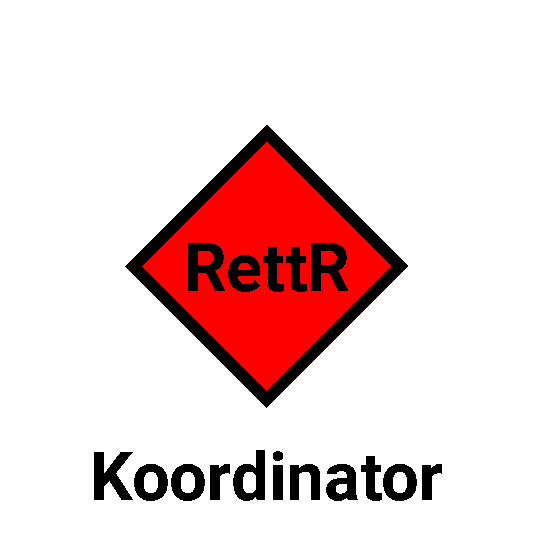
\includegraphics[width=0.15\linewidth]{images/RettR_p_Koordinator.pdf} & 
\includegraphics[width=0.15\linewidth]{images/RettR_p_atm.pdf} & 
\includegraphics[width=0.15\linewidth]{images/RettR_p_wtm.pdf} & 
\includegraphics[width=0.15\linewidth]{images/RettR_p_stm.pdf}
\\

\includegraphics[width=0.15\linewidth]{images/RettR_p_Gruppenfuehrer.pdf} & 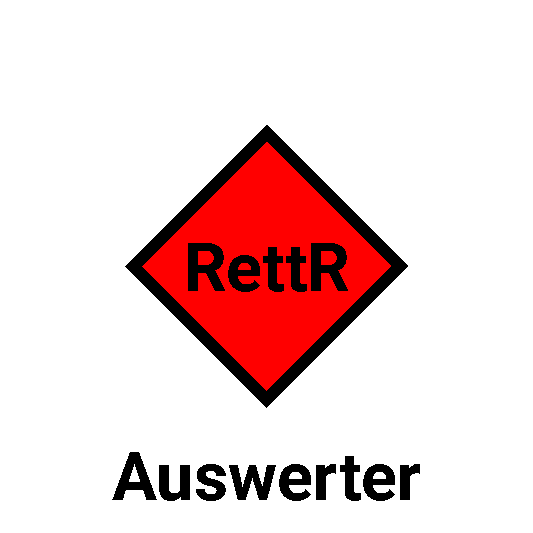
\includegraphics[width=0.15\linewidth]{images/RettR_p_Auswerter.pdf} & 
\includegraphics[width=0.15\linewidth]{images/RettR_p_atf.pdf} & 
\includegraphics[width=0.15\linewidth]{images/RettR_p_wtf.pdf} & 
\includegraphics[width=0.15\linewidth]{images/RettR_p_stf.pdf}
\\
\\ \hline
& & \angriffstrupp{} & \wassertrupp{} & \schlauchtrupp{}

\end{tabular}
\end{table}

\subsubsection{Führung}

Der \gruppenfuehrer{} übernimmt die Führung der Gruppe sowie die Beratung der Einsatzleitung.\\

\noindent Die Ausrüstung umfasst die persönlichen Schutzausrüstung sowie ein \ac{hrt} (TMO, nach Vorgabe).

\subsubsection{\melder}

Der \melder{} dokumentiert den Einsatz und koordiniert die Aufträge der Einsatzmittel für eigene oder dritte Kräfte nach Maßgabe des Gruppenführers.\\

\noindent Die Ausrüstung umfasst die persönlichen Schutzausrüstung sowie zwei \ac{hrt} oder \acp{mrt} (TMO, nach Vorgabe und \acs{dmo}, \dmoGroup{}).

\subsubsection{\maschinist}

Der \maschinist{} ist für die Aufbereitung und Kommunikation der gewonnen Informationen für die Einsatzleitung verantwortlich.\\

\noindent Die Ausrüstung umfasst die persönlichen Schutzausrüstung sowie ein \ac{hrt} (\acs{dmo}, \dmoGroup{}).

\subsubsection{\robotiktrupp}

Der \robotiktrupp{} ist für die Steuerung der Einsatzmittel verantwortlich. Der Trupp gliedert sich in Fernpilot:in und Einsatzraumbeobachter:in.\\

\noindent Die Ausrüstung umfasst jeweils die persönlichen Schutzausrüstung sowie ein \ac{hrt} (\acs{dmo}, \dmoGroup{}) sowie die vorgegebenen Einsatzmittel.\\

\noindent Die Aufgabe des Fernpiloten umfasst die Steuerung der Einsatzmittel. Der Einsatzraumbeobachter kontrolliert das Umfeld des Einsatzraums und übernimmt, wenn nicht anderweitig abgedeckt, die Dokumentation des Einsatzes.

\subsubsection{\schlauchtrupp}

Der \schlauchtrupp{} stellt die Arbeitsfähigkeit im Einsatz sicher. Der Trupp kümmert sich um das Akkumanagement und stellt die Verbindung zu anderen Einheiten (z. B. \ac{tel}) her. Im Verlauf des Einsatzes unterstützt der Trupp die \robotiktrupp{}s bei ihren Aufgaben.\\

\noindent Die Ausrüstung umfasst jeweils die persönlichen Schutzausrüstung sowie die vorgegebenen Einsatzmittel.

\subsection{Qualifikationen}
\label{sec:qualifikationen}

Alle Mitglieder der \callee{} verfügen mindestens über folgende Qualifikationen und Fortbildungen:

\begin{itemize}
 \item Ausbildung zum \textit{Truppmann Teil 1} und \textit{Teil 2} entsprechend FwDV 2, Kapitel 2.1
 \item Ausbildung zum \textit{Sprechfunkter} entsprechend FwDV 2, Kapitel 3.1
 \item EU-Kompetenznachweis A1\,/\,A3 \flq kleiner Drohnenführerschein\frq{}
\end{itemize}

\noindent Eine Mitgliedschaft in der \callee{} ist, ohne die Mindestanforderungen zu erfüllen, unter Vorbehalt möglich. Diese sind nach Eintritt in die \callee{} schnellstmöglich nachzuweisen. Bis zum Erbringen der Nachweise ist ausschließlich eine Teilnahme an Ausbildungsdiensten zugelassen.\\

\noindent In der \callee{} sollten folgende Qualifikationen und Fortbildungen durch einige Mitglieder abgedeckt werden:

\begin{itemize}
 \item Ausbildung zum \textit{Maschinisten} entsprechend FwDV 2 Kapitel 3.3
 \item Ausbildung zum \textit{Truppführer} entsprechend FwDV 2 Kapitel 2.2
 \item EU-Kompetenznachweis A2 \flq großer Drohnenführerschein\frq{}
\end{itemize}

\noindent Die Funktion des \gruppenfuehrer{}s sowie des stellvertretenden \gruppenfuehrer{}s setzt folgende Qualifikationen und Fortbildungen voraus:

\begin{itemize}
 \item Ausbildung zum \textit{Gruppenführer} entsprechend FwDV 2 Kapitel 4.1
 \item EU-Kompetenznachweis A2 \flq großer Drohnenführerschein\frq{}
\end{itemize}

\noindent Weitere Qualifikationen und Fortbildungen der Mitglieder sind wünschenswert. Ein Anspruch auf die Zuteilung von Lehrgängen durch den Landkreis besteht nicht. Ausgenommen hiervon sind die Lehrgänge für Führungskräfte der \callee{}. Die Kosten für den EU-Kompetenznachweis A1\,/\,A3 sowie EU-Kompetenznachweis A2 werden durch den Landkreis \district{} getragen.

\subsection{Organisation im Dienstbetrieb}

Für die \callee{} ist die Schaffung von Dienststellungen vorgesehen, um einen geregelten Dienst- und Ausbildungsbetrieb zu ermöglichen. Den benannten Personen ist der Zugang zu notwendigen Informationen sowie Räumlichkeiten der Feuerwehr oder des Landkreises im Rahmen der Dienstausübung zu gewähren.

\subsubsection{\gruppenfuehrer{}}

Der \gruppenfuehrer{} ist für die \callee{} verantwortlich und vertritt diese mit allen Belangen nach außen. Die Tätigkeiten im Dienstbetrieb umfassen:

\begin{itemize}
 \item halbjährliches Erstellen der Dienstpläne,
 \item Festlegen der inhaltlichen Ziele der Ausbildung,
 \item Durchführen der Ausbildung,
 \item Aufstellen der Materialanforderungen sowie
 \item alle weiteren Tätigkeiten, die der Umsetzung dieses Konzepts dienlich sind.
\end{itemize}

\subsubsection{stellvertretender \gruppenfuehrer{}}

Der stellvertretende \gruppenfuehrer{} unterstützt den \gruppenfuehrer{} bei den genannten Aufgaben und vertritt diesen, wenn dies notwendig sein sollte.\\

\noindent Kann der \gruppenfuehrer{} länger als sechs Monate den Dienstbetrieb nicht fortführen, übernimmt der stellvertretende \gruppenfuehrer{} nach Feststellung des Umstands die Position des \gruppenfuehrer{}s unverzüglich kommissarisch. Die kommissarische Führung der \callee{} darf sich auf maximal ein Jahr erstrecken.

\subsubsection{Gerätewart}

Der Gerätewart ist für die Pflege und Wartung der Einsatzmittel verantwortlich. Darüber hinaus unterstützt er bei der Dokumentation von dokumentationspflichtgen Tätigkeiten, z.\,B. der Dokumentation von Flugstunden der Mitglieder.

\subsection{Organisation an Einsatzstellen}

Bei der gemeinsamen Alarmierung mit weiteren Einheiten der \unit{} untersteht die Führung der \callee{} organisatorisch immer dem Zug- oder Bereitschaftsführer.\\

\noindent Andernfalls untersteht die \callee{} der Einsatzleitung in Form einer Stabsstelle. Ist am Einsatzort ein \ac{elw} oder eine \ac{tel} tätig, unterstützt die \callee{} die Arbeit der jeweiligen Besatzung.

\subsection{Taktische Zeichen}

Zur Lagedarstellung in \ac{elw} oder \ac{tel} sind der \callee{} taktische Zeichen entsprechend der Empfehung des BBK Empfehlungen für \flq Gemeinsame Regelungen zum Einsatz von Drohnen im Bevölkerungsschutz\frq{}\footnote{\url{https://www.bbk.bund.de/SharedDocs/Downloads/DE/Mediathek/Publikationen/Krisenmanagement/drohnen-empfehlungen.pdf;jsessionid=6D0A95E6A14ED029BCE3A30BB788273D.live362?__blob=publicationFile&v=8}}, S. 19 zugewiesen.\\

\noindent Taktische Zeichen für Führungskräfte\,/\,Führungsgehilfen und Personen mit Sonderfunktionen entsprechen den \flq Empfehlungen für taktische Zeichen im Bevölkerungsschutz\frq{}\footnote{\url{https://www.bildungsinstitut-rlp.drk.de/fileadmin/Download/Fuehrungskraefte/Ausbildung/ZF-Ausbildung/Empfehlungen_Takt_Zeichen_im_BevSch.pdf}}.\\

\noindent Eine Umsetzung der taktischen Zeichen als Vectordateien steht im Git-Repository von Jonas Köritz  unter \href{https://github.com/jonas-koeritz/Taktische-Zeichen}{https://github.com/jonas-koeritz/Taktische-Zeichen} zur Verfügung.\\

\noindent Die folgenden taktischen Zeichen zeigen sowohl das taktische Zeichen für eine Gruppe, sowie einen Trupp. Auf Grundlage des vorliegenden Konzeptes ist die Verwendung des taktischen Zeichens einer Gruppe vorzuziehen.

\begin{figure}[h!]
  \centering
  \subfloat[][Gruppe]{
\includegraphics[width=0.15\linewidth]{images/RettR_Gruppe.pdf}}
  \qquad
  \subfloat[][Trupp]{
\includegraphics[width=0.15\linewidth]{images/RettR_Trupp.pdf}}
\end{figure}
